\section{Finite laws, posterior motion, and the proof architecture}\label{sec:setup}

We first allow the policy to know a finite input law. This permits
conditional distributions of an offline optimum, while still forbidding
the policy from observing the realized future. The estimate obtained in
this setting must have an additive term uniform in the law and horizon.
Section~\ref{sec:transfer} uses precisely this uniformity to construct
one policy on an arbitrary metric.

\subsection{Matching and lazy simulation}

A configuration is a multiset of \(k\) points, with each repeated
point counted separately. For two configurations \(A=(a_1,\ldots,a_k)\)
and \(C=(c_1,\ldots,c_k)\), put
\[
 \mathsf M(A,C)=\min_{\pi\in S_k}\sum_{i=1}^k d(a_i,c_{\pi(i)}).
\]
This distance ignores the labels when matching configurations; an
actual server retains its label when it moves. A \emph{simulated}
configuration may move several members between requests. Its movement
cost is the matching distance between its successive configurations.
A policy is \emph{strongly lazy} if it does nothing when a server already
occupies the request, and otherwise moves exactly one server to it.

The classical cost-nonincreasing lazy reduction for the same starting
configuration is due to Manasse, McGeoch, and Sleator
\cite[Lemma~1, p.~211]{MMS90}. The matching-potential formulation below
also permits an arbitrary initial mismatch.

\begin{lemma}[Lazy simulation]\label{lem:lazy-simulation}
Suppose a causal sequence of simulated configurations
\(C_0,C_1,\ldots,C_H\) contains the request \(r_t\) at each time
\(t\ge1\). From any actual start \(A_0\), a strongly lazy policy serves
the same requests and satisfies, pathwise,
\[
 \cost(A_0;r_1,\ldots,r_H)
 \le \mathsf M(A_0,C_0)+\sum_{t=1}^H\mathsf M(C_{t-1},C_t).
\]
The conclusion also holds if the matching distances on the right are
replaced by any larger specified movement costs.
\end{lemma}

\begin{proof}
After \(C_t\) is revealed, take a minimum matching from \(A_{t-1}\)
to \(C_t\). If \(A_{t-1}\) does not contain \(r_t\), move the actual
server matched to a chosen occurrence of \(r_t\) in \(C_t\) to that
point. Keeping the same matching after the move shows that
\[
 \text{actual cost at }t+\mathsf M(A_t,C_t)
 \le \mathsf M(A_{t-1},C_t).
\]
If the request was already covered, make no move and the inequality
holds with equality. Composing minimum matchings gives
\[
 \mathsf M(A_{t-1},C_t)
 \le \mathsf M(A_{t-1},C_{t-1})
       +\mathsf M(C_{t-1},C_t).
\]
Summing and discarding the nonnegative final matching distance proves
the claim. Minimum matchings exist because there are only \(k!\)
permutations, even with repeated positions. Fixed orders resolve all
ties, so this procedure is causal.
\end{proof}

The same pathwise inequality applies to any prescribed simulated
trajectory. Causality is needed to obtain an online policy from it;
when comparing two offline optima, only the pathwise inequality is
used.

We use the shorthand
\[
                         \ell=1+\log(k+1).
\]
All unnamed multiplicative constants below are absolute. Constants may
depend on numerical parameters only after those parameters have been
fixed once and for all, independently of \(k\) and the metric.

\begin{proposition}[Finite distributional estimate]\label{prop:finite-law}
There is an absolute \(a<\infty\) with the following property. For every
finite metric \(Y\) of positive diameter, every \(k\ge2\), and every
start \(s\in Y^k\), there is a finite \(D_0=D_0(Y,k,s)\) such that,
for every finite horizon \(H\) and every probability law on \(Y^H\),
there is a causal strongly lazy policy satisfying
\begin{equation}\label{eq:finite-law}
             \E\,\cost\le a\ell^2\E\,\OPT+D_0 .
\end{equation}
The policy may depend on the law and horizon. The number \(D_0\)
does not.
\end{proposition}

Sections~\ref{sec:allocation}--\ref{sec:rounding} prove this
proposition. An additive term in those sections is always bounded by
a fixed finite function of \(Y,k,s\) and the finite structures
constructed from them. It never depends on the law, horizon, number
of histories, or number of updates. We will verify this distinction
again when assembling the estimates.

\subsection{Hidden comparators and the two parts of a posterior update}

Fix the data of Proposition~\ref{prop:finite-law}. For each input,
choose one optimum trajectory of the \(k\) labeled servers, resolving
ties by a fixed order. Such a choice exists: each request has only
\(k\) possible server labels, so a length-\(H\) input has only \(k^H\)
candidate trajectories. The chosen optimum is a hidden random variable
determined by the input. Set
\[
                         Q=\E\,\OPT .
\]
The policy uses conditional laws of this trajectory, not its hidden
realization.

Let \(\mathcal F_t\) contain the request prefix through time \(t\)
and the independent random tape used to construct the partitions.
It is convenient to include that entire tape from time zero. The
rounding procedure will use a separate independent tape that is
excluded from \(\mathcal F_t\). Thus conditioning on \(\mathcal F_t\)
does not alter the true-metric comparator posterior beyond
conditioning on the request prefix.

For any old hidden quantity \(Z_{t-1}\), a step has two logically
different parts:
\[
 \mathcal L(Z_{t-1}\mid\mathcal F_{t-1})
 \xrightarrow{\mathrm{filtering}}
 \mathcal L(Z_{t-1}\mid\mathcal F_t)
 \xrightarrow{\mathrm{drift}}
 \mathcal L(Z_t\mid\mathcal F_t).
\]
Here \(\mathcal L\) denotes a probability law, not the pilot potential
introduced later. During filtering, an affine functional with
coefficients held from time \(t-1\) has zero conditional expected
change. A concave functional has nonpositive conditional expected
change. During drift, the joint conditional law of
\((Z_{t-1},Z_t)\) provides a coupling. For embedded quantities, the
old variable uses the old map and the new variable uses the new map.

All signed filtering estimates are applied over every step, with old
parameters held fixed, \emph{before} selecting resets or partition
edits. In particular, no argument conditions a martingale estimate on
the later event that a reset is necessary.

For probability estimates concerning random radii or retirements, we
use a different conditioning: fix the true input and its comparator
trajectory, and average over the partition tape. The relevant
insertion schedules will then be deterministic. This does not assert
independence after conditioning on the entire tape in \(\mathcal F_t\).

At a fixed finite horizon all relevant random outcomes can be taken
finite. A radius draw need only specify which subset of the finite
space is its ball; a roster lifetime has a finite maximum age.
Only finitely many insertions can occur. More explicitly, preallocate
at most \(H\) insertion slots per level and structure, discretize each radius
at all pairwise distances in \(Y\), and preallocate each entry's
truncated lifetime. This gives a finite-valued relevant tape, even
before the centers of the inserted balls are known. Any unused
portion of an ambient infinite tape is independent and can be ignored;
all fractional states and selected rounding kernels below depend only
on this finite projection and the request prefix. Realizing a kernel
also uses the current rounded state and the independent rounding
randomness. Conditional laws, minimizing choices, and randomized rounding
kernels can therefore be specified
history by history. Arbitrary continuations are assigned to
zero-probability histories.

\subsection{The true-metric measure update}

Write \(x=r_t\), and designate the server moved by the chosen optimum
at this request, including when its movement is zero. Let
\(\mu^{\mathrm{old}}\) be the expected comparator counting measure
at time \(t-1\), conditional on \(\mathcal F_{t-1}\). At the new
conditioning \(\mathcal F_t\), let \(\mu^-\) and \(\mu^+\) be its
counting measures before and after the move, and let \(\nu\) be the
probability law of the designated mover's old position. Then
\begin{equation}\label{eq:measure-update}
 \mu^+=\mu^--\nu+\delta_x,\qquad
 \nu\le\mu^-,\qquad \nu(Y)=1,\qquad
 e_x=\int_Y d(x,y)\,d\nu(y).
\end{equation}
Both counting measures have total mass \(k\), the measure \(\mu^+\)
has at least one unit at \(x\), and
\[
 \E[\mu^-\mid\mathcal F_{t-1}]=\mu^{\mathrm{old}},
 \qquad
 \E\sum_{t=1}^H e_{r_t}=Q.
\]
The expected counting measure of the stationary members is
\(\mu^+-\delta_x=\mu^--\nu\), hence is bounded by \(\mu^+\).
The separate treatment of this stationary measure and the designated
mover will matter in the partition accounting.

\subsection{Scales and a logarithmic telescope}

Balls are closed. Set \(r_0=\diam Y\) and
\[
 r_j=r_0\tau^{-j},\quad 1\le j\le J,\qquad
       40r_J<\min_{p\ne q}d(p,q).
\]
The separation factor \(\tau\ge2\) is a sufficiently large absolute
constant. Its required lower bounds come from tree allocation and
rounding; neither bound depends on \(k,Y,J\). Once it is fixed,
\(J\) depends only on \(Y\).

\begin{lemma}[Ball-mass telescope]\label{lem:scale-logarithms}
Fix \(0<a<b\), a nonnegative measure \(\mu\), and an offset \(c_0\ge0\).
On a consecutive finite interval of scale indices suppose
\[
 c\le A_j:=c_0+\mu(B(x,ar_j))
 \le B_j:=c_0+\mu(B(x,br_j))\le K,
 \qquad c>0.
\]
If \(p\ge1\) is an integer with \(\tau^p a\ge b\), then
\[
                  \sum_j\log(B_j/A_j)\le p\log(K/c).
\]
\end{lemma}

\begin{proof}
Extend \(A_j\) before the coarsest index of the interval by the value
\(K\). Ball inclusion gives \(B_j\le A_{j-p}\) whenever the shifted
index remains in the interval, and the same inequality follows from
\(B_j\le K\) at the coarse boundary. Thus the sum is at most
\(\sum_j(\log A_{j-p}-\log A_j)\). All interior terms cancel, leaving
at most \(p\) coarse-end terms minus at most \(p\) fine-end terms.
Each resulting difference is at most \(\log(K/c)\).
\end{proof}

In every application, \(a,b,c\) are fixed positive constants and
\(K=O(k+1)\), so the bound is \(O(\ell)\). The offset permits its use
with \(1+\mu(B)\) as well as with positive ball masses themselves.
Geometric sums of radii, by contrast, cost an absolute multiple of
their largest radius and introduce no logarithm.

\subsection{Where the two logarithms occur}

The allocation theorem begins with a fixed finite tree and a hidden
trajectory of \(k\) members on its leaves. It constructs subtree
amounts \(q_v\) satisfying
\[
 q_{\mathrm{root}}=k,\qquad
 \sum_{i\text{ child of }v}q_i\le q_v,\qquad
                    q_v\le C_0m_v,
\]
where \(m_v\) is the posterior expected hidden subtree count.
The inequality in conservation allows \emph{parking} at internal
vertices:
\[
                  p_v^\circ=q_v-\sum_iq_i .
\]
All parks together have total mass \(k\). This freedom is useful:
the required leaf still receives at least one unit, but unused mass
need not follow rapidly changing posterior proportions down the tree.
Figure~\ref{fig:parked-tree} illustrates this split and the separate
movement of its representative.

The construction order is important. Partition schedules use only the
true-metric posteriors and chronological ages. They are independent of
the later allocation and rounding. Their bounded simultaneous
occupancy gives a finite set of labels, chosen independently of the
horizon. Full strings of level labels then define a fixed finite
prefix tree. We apply the allocation theorem to that tree, control
the moving representatives using the domination \(q_v\le C_0m_v\),
and round with a further independent tape. Finally
Lemma~\ref{lem:lazy-simulation} returns to the original one-server
movement model.

\begin{figure}[!htbp]
 \centering
 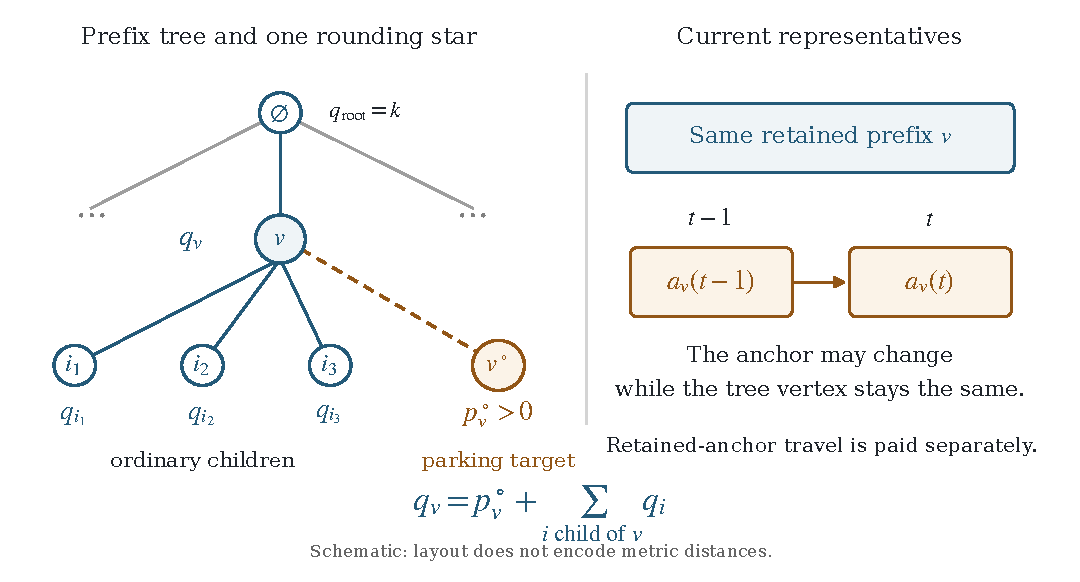
\includegraphics[width=.94\textwidth]{figures/parked_tree.pdf}
 \caption{A subtree amount is split between its children and a park at
 its own vertex. The park is included as one more child target during
 rounding. A fixed tree vertex can have a moving representative in
 the original metric, so its parked mass requires a separate travel
 estimate. The picture records conservation and does not assert that
 the original metric is a Euclidean tree.}
 \label{fig:parked-tree}
\end{figure}

Let \(P\) be expected movement of the mapped hidden comparator on tree
leaves, and put
\[
       V=\E\sum_t\sum_{v\ne\mathrm{root}}
                     r_{|v|-1}|\Delta q_v|.
\]
The main estimates are
\begin{align*}
 P&\le C\ell Q+B_P,\\
 V&\le C\ell P+B_V,\\
 \E\,\cost_{\mathrm{sim}}
   &\le C(V+\ell P+\ell Q)+B_T.
\end{align*}
Their additive terms have the uniform meaning specified above.
Figure~\ref{fig:budget-flow} displays their dependence.

\begin{figure}[!htbp]
 \centering
 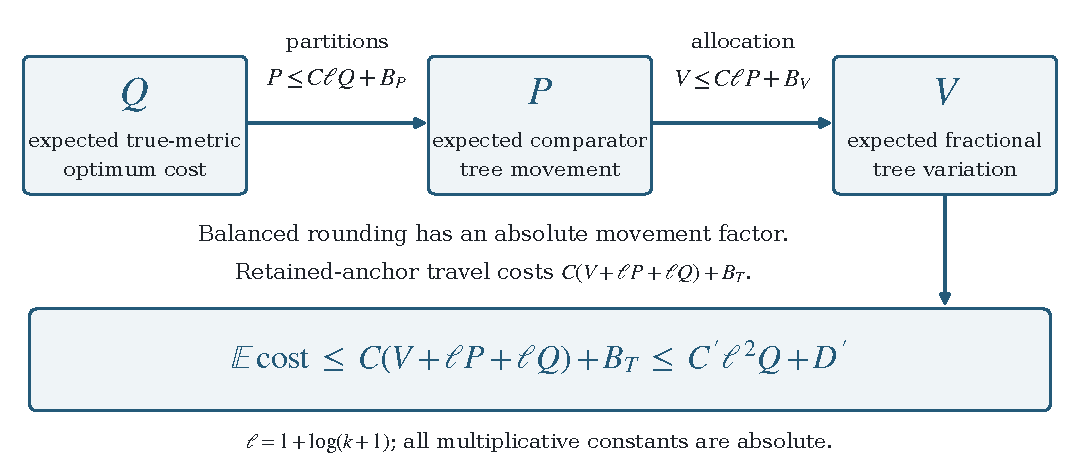
\includegraphics[width=.98\textwidth]{figures/budget_flow.pdf}
 \caption{Movement accounting. The partitions and the tree allocation
 each contribute one logarithm. Rounding has an absolute loss.
 Moving the representatives costs \(O(V+\ell P+\ell Q)\), so it
 preserves the final squared logarithm. All additive terms shown
 are uniform in the finite input law and horizon.}
 \label{fig:budget-flow}
\end{figure}

